% \subsection{Động lực của tiến hóa đa nhiệm}
% Với sự phát triển của EA các nhà nghiên cứu đã và đang tiếp tục đưa ra những hướng nghiên cứu mới, những thuật toán hiệu quả cao hơn. Trong những năm gần đây, \emph{tiến hóa đa nhiệm} nổi lên như là một xu hướng trong cộng đồng các nhà nghiên cứu \emph{thuật toán tiến hóa} và \emph{tính toán thông minh}. Không chỉ một mà nhiều bài toán tối ưu có thể được giải quyết cùng nhau, điều này còn được gọi với cái tên khác là \emph{tối ưu hóa đa tác vụ} (thuật ngữ gốc: \emph{multitask  optimization}.

Trong khoa học máy tính và học máy có một thuật ngữ được gọi là \emph{học đa nhiệm vụ } (thuật ngữ gốc: \emph{multitask learning}) nó khá tương đồng với \emph{multitask  optimization}. Trong \textbf{multitask learning} các tác vụ liên quan sẽ chia sẻ kiến thức với nhau, và được huấn luyện cách đồng thời. Lấy ví dụ trong hệ thống phân loại email rác, có thể coi đây là các tác vụ phân loại riêng biệt nhưng có liên quan giữa các người dùng với nhau. Cụ thể hơn, những người khác nhau sẽ có những cơ chế, đặc tính phân loại tin email và email thường khác nhau. Tuy nhiên, hầu hết người dùng đều không tự gán nhãn đủ để có thể xây dựng cơ chế đủ tốt phân loại email cá nhân hóa, trong khi dữ liệu lại quá nhiễu để sử dụng cơ chế phân loại chung cho tất cả các người dùng. Bởi vậy kỹ thuật \textbf{multitask learning} sẽ dựa vào thông tin từ những người dùng thường xuyên gán nhãn email để làm cơ sở kiến thức trong việc xây dựng cơ chế cá nhân hóa cho các người dùng khác. Trong khi đó, \textbf{multitask  optimization} cũng giúp các tác vụ được tối ưu một cách đồng thời nhưng là một thuật ngữ chung hơn, nó không phụ thuộc vào việc các thông tin trong mô hình được kết nối với nhau như thế nào để chia sẻ. Mà nó giúp giữa các tác vụ có liên quan đến nhau có thể chia sẻ không gian giải pháp với tác vụ khác để đẩy tốc độ tìm kiếm giải pháp tối ưu trên tác vụ đó, bao gồm cả các giải pháp rời rạc và tối ưu. 

Để cụ thể hơn, lấy ví dụ bài toán \emph{dịch vụ đám mây theo yêu cầu} (thuật ngữ gốc: \emph{cloud-based-on-demand}) cung cấp cho khách hàng sử dụng. Có thể hiểu là hệ thống sẽ phải giải quyết nhiều tác vụ tối ưu cùng lúc được nhận từ nhiều người dùng vào cùng một thời điểm. Mỗi tác vụ có thể có những đặc tính chung nào đó hoặc chúng hoàn toàn khác nhau. Nói một cách khác \textbf{multitask optimization} có thể được xem như là một mô thức chung trong việc giải quyết các bài toán tối ưu hóa. Không chỉ là việc chia sẻ kiến thức 1 chiều từ những tác vụ đơn giản đến tác vụ phức tạp, mà thực tế khi giải quyết những tác vụ phức tạp sẽ có thể giải quyết được những tác vụ đơn giản hơn. 

Một cách tiếp cận \empth{tiến hóa} cho \empth{multitask optimization} được gọi là \empth{evolutionary multitasking} hay còn gọi là tiến hóa đa tác vụ. Nó là một phương pháp kết hợp tư tưởng của thuật toán EA theo hướng tối ưu hóa nhiều vấn đề một cách đồng thời dựa theo cơ sở của lý thuyết \empth{multitask optimization}.
% \begin{figure}[ht]
%     \centering
%     \fbox{
\includegraphics[width=0.6\linewidth]{mindfulness.jpg}}
%     \caption{Mô tả về đa nhiệm của nhận thức khi bộ não liên tục phải nhận nhiều tín hiệu từ các nguồn khác nhau và xử lý chúng đồng thời}
%     \label{fig:mfea:cognitive-multitasking}
% \end{figure}

Bên cạnh đó, tiến hóa đa nhiệm còn lấy cảm hứng ý tưởng từ tưởng, não của con người có thể giải quyết được nhiều tác vụ cùng một lúc. Lấy ví dụ, con người thường hay nói chuyện khi đi bộ, nghe nhạc khi đang học, vừa hát vừa đánh đàn vv.. các công việc này đều yêu cầu não bộ phải xử lý các thông tin khác nhau từ các tác vụ khác nhau. Một đứa trẻ khi lớn lên đã phải có khả năng giải quyết nhiều việc cùng một lúc, học nhiều môn học, học nhiều thứ tiếng. Việc giải quyết nhiều tác vụ cùng một lúc giờ đây là điều tất nhiên con người phải thích nghi để sống sót, tồn tại trong xã hội. So với trước đây, não bộ con người ngày càng được yêu cầu cao hơn, đòi hỏi phải xử lý nhiều thông tin hơn. Có một điểm cần lưu ý là tuy não bộ con người giải quyết nhiều tác vụ cùng một lúc, tuy nhiên khi chuyển từ tác vụ này sang tác vụ khác, nó có khả năng tái sử dụng những kinh nghiệm đã học được từ tác vụ trước đó để giải quyết tác vụ tiếp theo. 
\subsection{Tối ưu hóa đa nhiệm}
Trong những năm gần đây mô hình tối ưu đa nhiệm (thuật ngữ gốc: Multifactorial Optimization - \emph{MFO}) đã lần đầu được đề xuất bởi Ong and Gupta trong bài báo \cite{ong2016evolutionary}. Lấy cảm hứng từ việc kiểm soát cùng lúc nhiều công việc trong cùng 1 thời điểm \cite{caruana1997multitask}. Ong and Gupta cho rằng các bài toán tối ưu hóa khác nhau có những điểm tương đồng nhất định mà việc giải quyết bài toán này có thể giúp bổ trợ cho bài toán kia. Dựa trên ý tưởng đó, họ đề xuất mô hình MFO trên cơ sở thực hiện việc tìm kiếm tập lời giải khả thi cho cùng lúc nhiều bài toán tối ưu hóa.
\begin{definition}
Bài toán \textbf{MFO}: cùng lúc cực tiểu hóa tập $K$ hàm $f_k(x^{(k)}), x^{(k)}\in \mathcal{X}_k \subset \mathbb{R}^n, k\in {1,2,...,K}$ ký hiệu là $\min_{x^{(k)}\in \mathbb{R}^n} f_k(x^{(k)})$. Trong đó:
\begin{itemize}
    \item $\min_{x^{(k)}\in \mathbb{R}^n}$ là biến quyết định của bài toán thứ $k$.
    \item $f_k(x): \mathcal{X}_k \rightarrow \mathbb{R}$ là hàm mục tiêu của bài toán thứ $k$.
    \item $\mathcal{X}_k$ là không gian tìm kiếm của bài toán thứ $k$
\end{itemize}
Mục tiêu của bài toán là tìm bộ lời giải tối ưu $(x^{(1)*},x^{(2)*}, x^{(3)*},...., x^{(K)*} )$ sao cho với mọi lời giải thành phần $x^{(k)*}$ ta có $f(x^{(k)*}) \leq f(x^{(k)}) \forall x^{(k)} \in \mathcal{X}_k$.
\end{definition}
Cụ thể trong MFO, ta cùng lúc đi tìm tập lời giải cho từng hàm tối ưu từng thành phần riêng lẻ. Cùng với việc đề xuất mô hình MFO. Ong and Gupta đã tiếp tục đề xuất các phương pháp so sánh lời giải trong không gian chung đa nhiệm và phát triển giải thuật tiến hóa đa nhiệm (thuật ngữ gốc: \emph{Multifactorial Evolution Algorithm - MFEA}) để giải quyết bài toán MFO nhằm tận dụng hiệu quả tìm kiếm của việc giải đồng thời các bài toán tối ưu hóa. Trong đồ án này tác giả sẽ gọi thuật toán MFEA là MFEA-I để phân biệt với thuật toán chính được nghiên cứu trong đồ án là giải thuật tiến hóa đa nhiệm với ước lượng hệ số trao đổi trực tuyến (thuật ngữ gốc: Multifactorial Evolution Algorithm with Online Transfer Parameter Estimation - MFEA-II)
\subsection{Tiến hóa đa nhiệm}
% Trước khi giải thích về thuật toán tối ưu hóa đa nhiệm 2 - MFEAII, tôi xin giải thích về nền tảng của nó, thuật toán tối ưu hóa đa nhiệm 1 - MFEAI
\label{mfeai}

Tiến hóa đa nhiệm như giải thích về MFO ở trên, MFEA-I áp dụng ý tưởng này để giải quyết một tập $K$ tác vụ đồng thời. Mỗi tác vụ $k \in \{1, ..., K\}$ sẽ có không gian tìm kiếm riêng là $X_k$ và hàm mục tiêu riêng là $F_k(x)$. Tuy nhiên MFEA-I chỉ sử dụng một quần thể để mã hóa toàn bộ $K$ không gian tìm kiếm đó. Do vậy tất cả các vật liệu di truyền từ các tác vụ khác nhau sẽ được mã hóa vào chung trong một không gian tìm kiếm chung. Các giải pháp từ các tác vụ khác nhau sẽ được đưa về một cấu trúc giống nhau để có thể sử dụng, kết hợp. Trong mỗi lần đánh giá, véc-tơ biểu diễn của tác vụ $k$ sẽ được giải mã từ không gian tìm kiếm chung về không gian tìm kiếm riêng của nó và tính giá trị của hàm mục tiêu. Một định nghĩa về không gian tìm kiếm chung thường được sử dụng đó là gán bằng giá trị của không gian tìm kiếm hay số chiều của tác vụ dài nhất. 

Một số định nghĩa quan trọng trong MFEA-I được đề xuất như sau:

\begin{definition}{\textbf{Giá trị thích nghi đơn nhiệm}} (thuật ngữ gốc: \emph{factorial cost}) $\Psi^i_j$ của cá thể $p_i$ đối với tác vụ cần tối ưu $T_j$ được tính bởi công thức $\Psi^i_j=\lambda\cdot\sigma^i_j +f^i_j$, với $\lambda$ là hệ số phạt lớn, $f^i_j$ và $\sigma^i_j$ lần lượt là giá trị hàm mục tiêu và tổng giá trị vi phạm ràng buộc tương ứng với mỗi $p_i$ và $T_j$. Theo đó $p_i$ là giải pháp khả thi với $T_j$ (giá trị vi phạm ràng buộc bằng 0), chúng ta có $\Psi^i_j=f^i_j$.
\label{def:factorial_cost}
\end{definition}

\begin{definition}{\textbf{Xếp hạng đơn nhiệm}} (thuật ngữ gốc: \emph{factorial rank}) $r^i_j$ của cá thể $p_i$ trên tác vụ $T_j$ đơn giản là chỉ số của $p_i$ trong danh sách các cá thể của quần thể được sắp xếp theo thứ tự giảm dần của $\Psi_j$.
\label{def:factorial_rank}
\end{definition}


Trong trường hợp $\Psi^a_j=\Psi^b_j$ với một cặp cá thể $p_a$ and $p_b$, có thể ngẫu nhiên lựa chọn để gán các giá trị \emph{xếp hạng đơn nhiệm}. Tuy nhiên vì hiệu suất của 2 cá thể là tương đương tại tác vụ $j^{th}$ nên ta sẽ gán nhãn nó như là đối tác $j$.
\begin{definition}{\textbf{Chỉ số kĩ năng}} (thuật ngữ gốc: \emph{skill factor}) $\tau_i$ của cá thể $p_i$ là một tác vụ trong số tất cả các tác vụ của MFO với điều kiện là cá thể $p_i$ có hiệu quả nhất trên tác vụ này. Công thức: $\tau_i = argmin_j{r^i_j}$ với $j \in {1, 2, ..., K}$
\label{def:skill_factor}
\end{definition}

\begin{definition}{\textbf{Độ thích nghi vô hướng}} (thuật ngữ gốc: \emph{scalar fitness}) $\phi_i$ của cá thể $p_i$ dựa vào danh sách các factorial ranks ${r^i_1, r^i_2, ..., r^i_K}$ của cá thể $p_i$ đối với tất cả các tác vụ. Công thức: $\varphi_{i}=1/\min_{j\in\{1,\ldots,K\}}\left\{r_{j}^{i}\right\}$.
\label{def:scalar_fitness}
\end{definition}

Trên cơ sở này Gupta, Ong and Feng đề xuất lược đồ giải thuật cho MFEA-I như hình \ref{mfea-flow} \cite{gupta2016multifactorial}.
\begin{figure}
    \centering
    \fbox{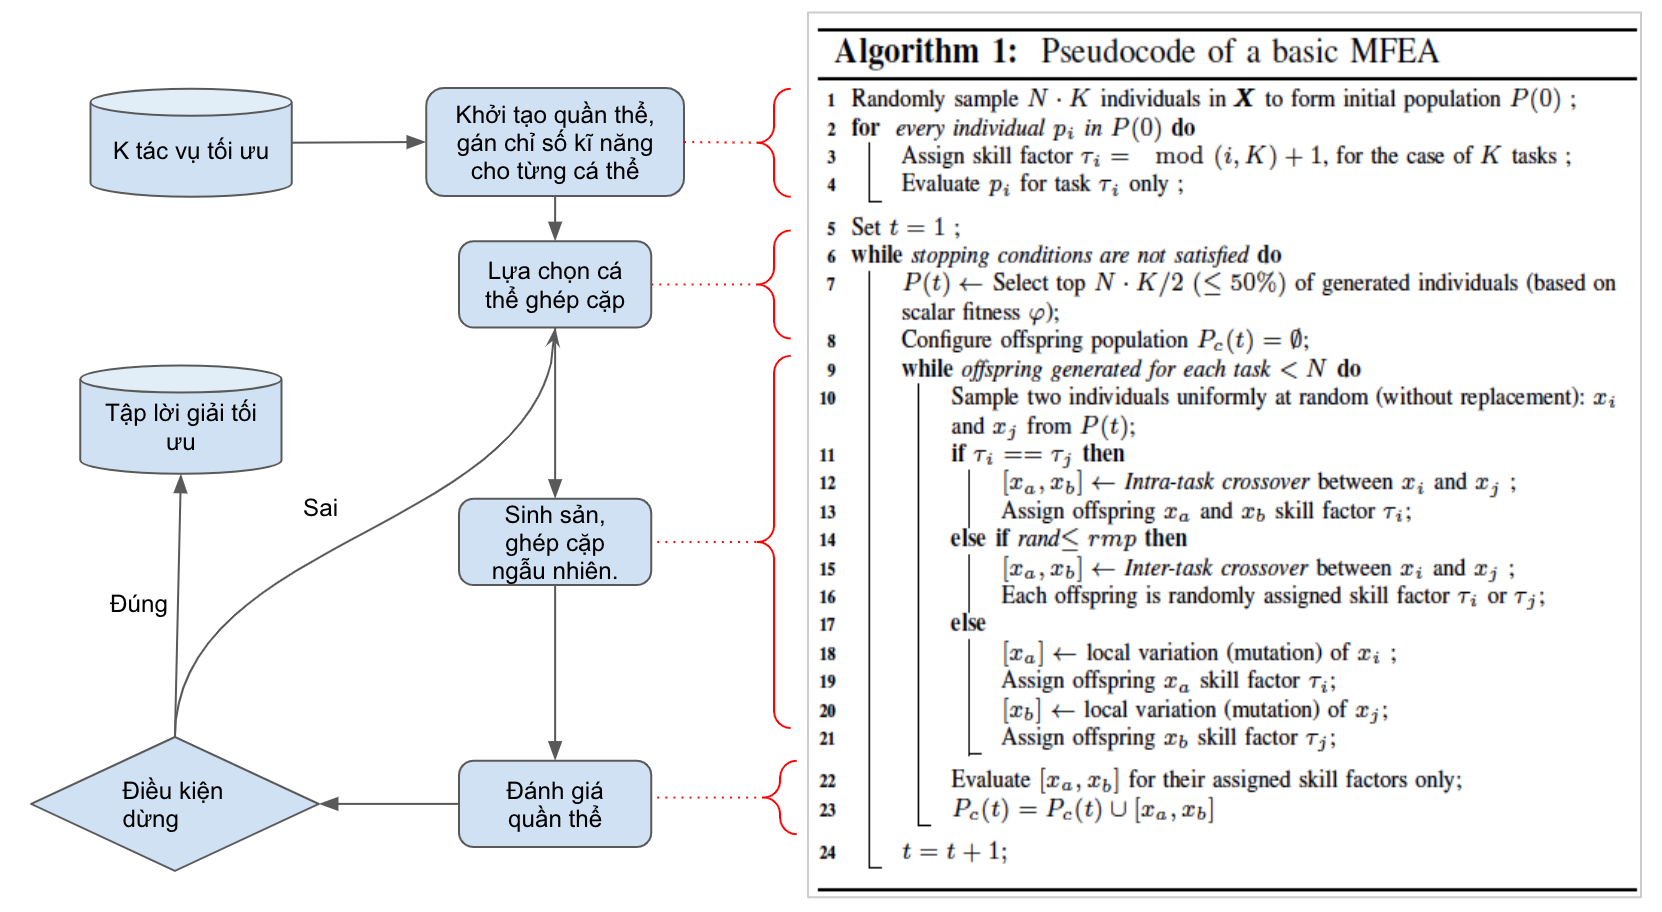
\includegraphics[width=0.85\linewidth]{thesis/images/mfea-alg.png}}
    \caption{Lược đồ giải thuật tiến hóa đa nhiệm MFEA-I \cite{gupta2016multifactorial}}
    \label{mfea-flow}
\end{figure}

Trong đó điểm khác biệt lớn nhất của MFEA-I so với thuật toán tiến hóa thông thường được mô tả tại \ref{section:cea} là cho phép lai ghép cá thể của các bài toán khác nhau theo một xác suất ghép cặp ngẫu nhiên (thuật ngữ gốc: \emph{random mating propability - rmp}). Phép lai ghép ngẫu nhiên đa nhiệm này đem đến một khả năng chia sẻ các gen tốt gữa các bài toán tối ưu hóa để đồng thời giải quyết cùng lúc chúng với tốc độ hội tụ nhanh hơn. 

Tuy nhiên, liệu việc kết hợp các lời giải của các bài toán tối ưu hóa khác nhau thì có sinh ra lời giải tốt hay không? Hoặc ít nhất cũng cần chỉ ra được trong trường hợp nào thì tốt, trường hợp nào thì không tốt. Các mục tiếp theo trong đồ án sẽ làm rõ hơn về vấn đề này.

